\documentclass[conference]{IEEEtran}
\IEEEoverridecommandlockouts
% The preceding line is only needed to identify funding in the first footnote. If that is unneeded, please comment it out.
\usepackage{cite}
\usepackage{amsmath,amssymb,amsfonts}
\usepackage{algorithmic}
\usepackage{graphicx}
\usepackage{float}
\usepackage{textcomp}
\usepackage{xcolor}
\usepackage{svg}
\usepackage{tabularx}

\def\BibTeX{{\rm B\kern-.05em{\sc i\kern-.025em b}\kern-.08em
    T\kern-.1667em\lower.7ex\hbox{E}\kern-.125emX}}
\begin{document}

\title{Evaluation of Cryptographic Protocols for Secure Communication in Artificial Pancreas Systems\\
{\footnotesize \textsuperscript{*}Note: Sub-titles are not captured in Xplore and
should not be used}
\thanks{Identify applicable funding agency here. If none, delete this.}
}

\author{\IEEEauthorblockN{\textsuperscript{} Suhasini Prakash}
\textit{Institute for Computing in Research}\\
Austin, Texas \\
hasinivp10@gmail.com}


\maketitle

\begin{abstract}
This paper explores the application of different cryptographic algorithms to a CGM/AID system. This specifically looks at the pipeline between the continuous glucose monitor and insulin pump/controller device (focusing on a hardware architecture where the controller is embedded within the insulin pump). Within the pipeline, this paper explores the security tradeoffs between various encryption mechanisms: comparing overall security, computational overhead, latency, and memory usage.
\end{abstract}


\section{Introduction}
Over 7.5 million people globally use continuous glucose monitoring devices (CGMs), many of whom also use a paired automated insulin delivery device (AIDs) (diabetesdata.org). Recently, security measures over these devices have gained more traction due to a rise in healthcare based cyber attacks and an increase in government regulation of healthcare devices.

\section{Background}

\subsection{Artificial Pancreas Systems}
Artificial pancreas systems are used by diabetes patients globally. Patients with diabetes are either unable to produce insulin regularly through their pancreas (Type 1) or are resistant to the absorption of insulin (Type 2). Almost all type 1 patients must artificially inject insulin in some way (such as using an artificial pancreas/insulin pump device), while some type 2 patients make use of such systems as well. These systems are used to mirror the function of healthy pancreas. An artificial pancreas system generally consists of a continuous glucose monitor (CGM), automated insulin device (AID) as well as a controller/algorithm which takes into account the current blood sugar readings, trend, food/physical activities, etc. to calculate the amount of insulin that needs to delivered to the patient [cite]. Most systems also have a smartphone/mobile device that allows for manual input of food/physical activity etc. It also acts as a method for the patient to view glucose readings, trends, and override the insulin pump as needed.

\subsection{High Level System Architectures}
There are various artificial pancreas system architectures: specifically regarding the placement of the controller algorithm. In many modern systems, the controller is embedded within the insulin pump itself in order to avoid the possibility of the insulin pump failing due to failed Bluetooth connection or damage to the mobile device. However, having the controller embedded in the insulin pump is not am FDA requirement, so there remain models where the controller remains in the smartphone/mobile device or as a separate device or entity. 

In this study, we are focusing on an architecture where the controller is embedded into the insulin pump device. 
\begin{figure}[H]
    \centering
    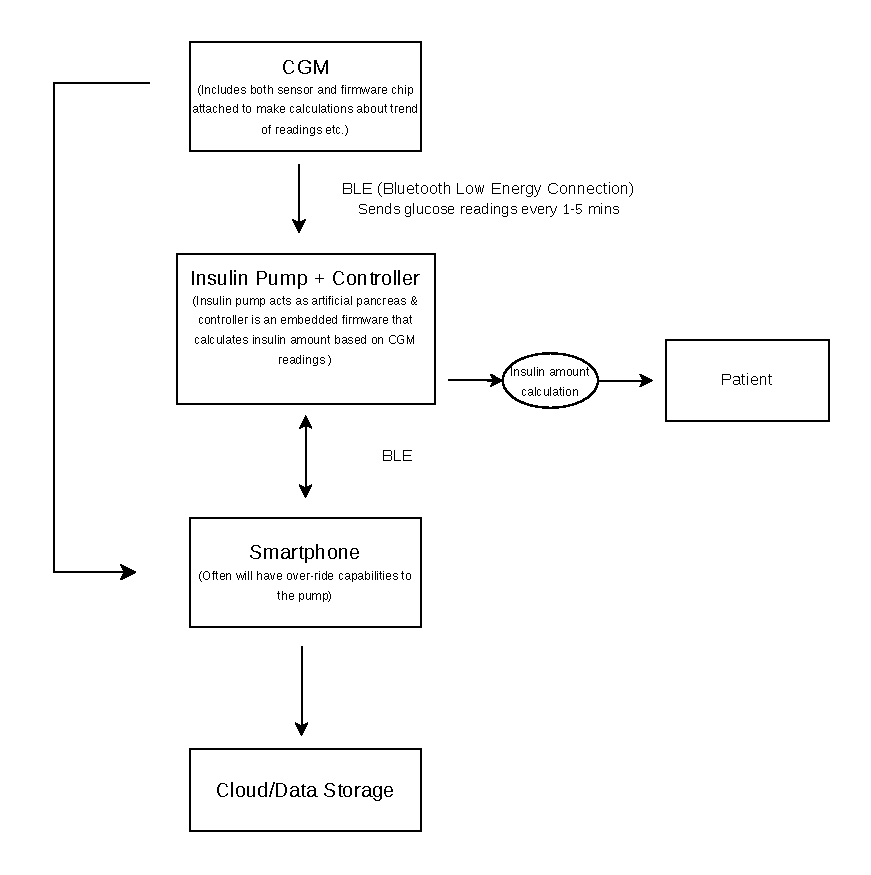
\includegraphics[width=1\linewidth]{HighLevelArchitecture.pdf}
    \caption{High Level System Architecture}
    \label{fig:placeholder}
\end{figure}

\subsection{STRIDE Threat Model}

In this study, an initial threat model was developed using the STRIDE threat modeling framework. Developed by Microsoft, this framework is used widely by cybersecurity professionals to categorize threats into one of 6 categories: (S) Spoofing, (T) Tampering, (R) Repudiation, (I) Information Disclosure, (D) Denial of Service, and (E) Elevation of Privilege.  

\subsection{STPA Sec Analysis Method}
STPA Sec is a security analysis framework developed at MIT that allows analysts to look at a system through a top-down lens focusing on control-feedback loops instead of analyzing vulnerabilities component by component. Moreover, this framework allows the analyst to understand how each failure in communication systems/feedback loops can lead to hazards/losses.

\subsection{Encryption Algorithms Evaluated}
\subsubsection{AES-CBC}
This is a basic algorithm that provides confidentiality through cipher block chaining using a random initialization vector (IV). This uses a block by block encryption mechanism, where before encrypting block N, it is XORed with block N-1. Because of it's block by block encryption nature, it uses padding (oftentimes PKCS-7) to ensure that the plaintext is a multiple of 16 bytes. This makes it vulnerable to padding-oracle and bit-flipping attacks.
\subsubsection{AES-CBC + HMAC}
This builds on the previous encryption algorithm by introducing an authentication mechanism via HMAC. HMAC is a hashing algorithm that acts on top of a key (MAC - Message Authentication Code) as a method to ensure integrity/authentication. By using this, the decryption algorithm can effectively verify that the data has not been tampered with. 
\subsubsection{AES-CCM}
This is the default algorithm used as a part of BLE connections (which most CGM/AID systems make use of). Through the use of AES-CTR (counter-mode), the CCM algorithm is able to mimic a stream-based encryption algorithm allowing for parallel processing.
\subsubsection{AES-GCM}
This modern AEAD encryption is often considered the standard for modern day security. 
\subsubsection{ChaCha20Poly1305}
This method is the most software-optimized algorithm, that is often used by DIY hackers/open source community.
\section{Methodology}
\subsection{STRIDE Threat Modeling}
In order to gain a better understanding of the potential threats, a STRIDE Threat Modeling of the system was conducted. 
\begin{figure}[H]
    \centering
    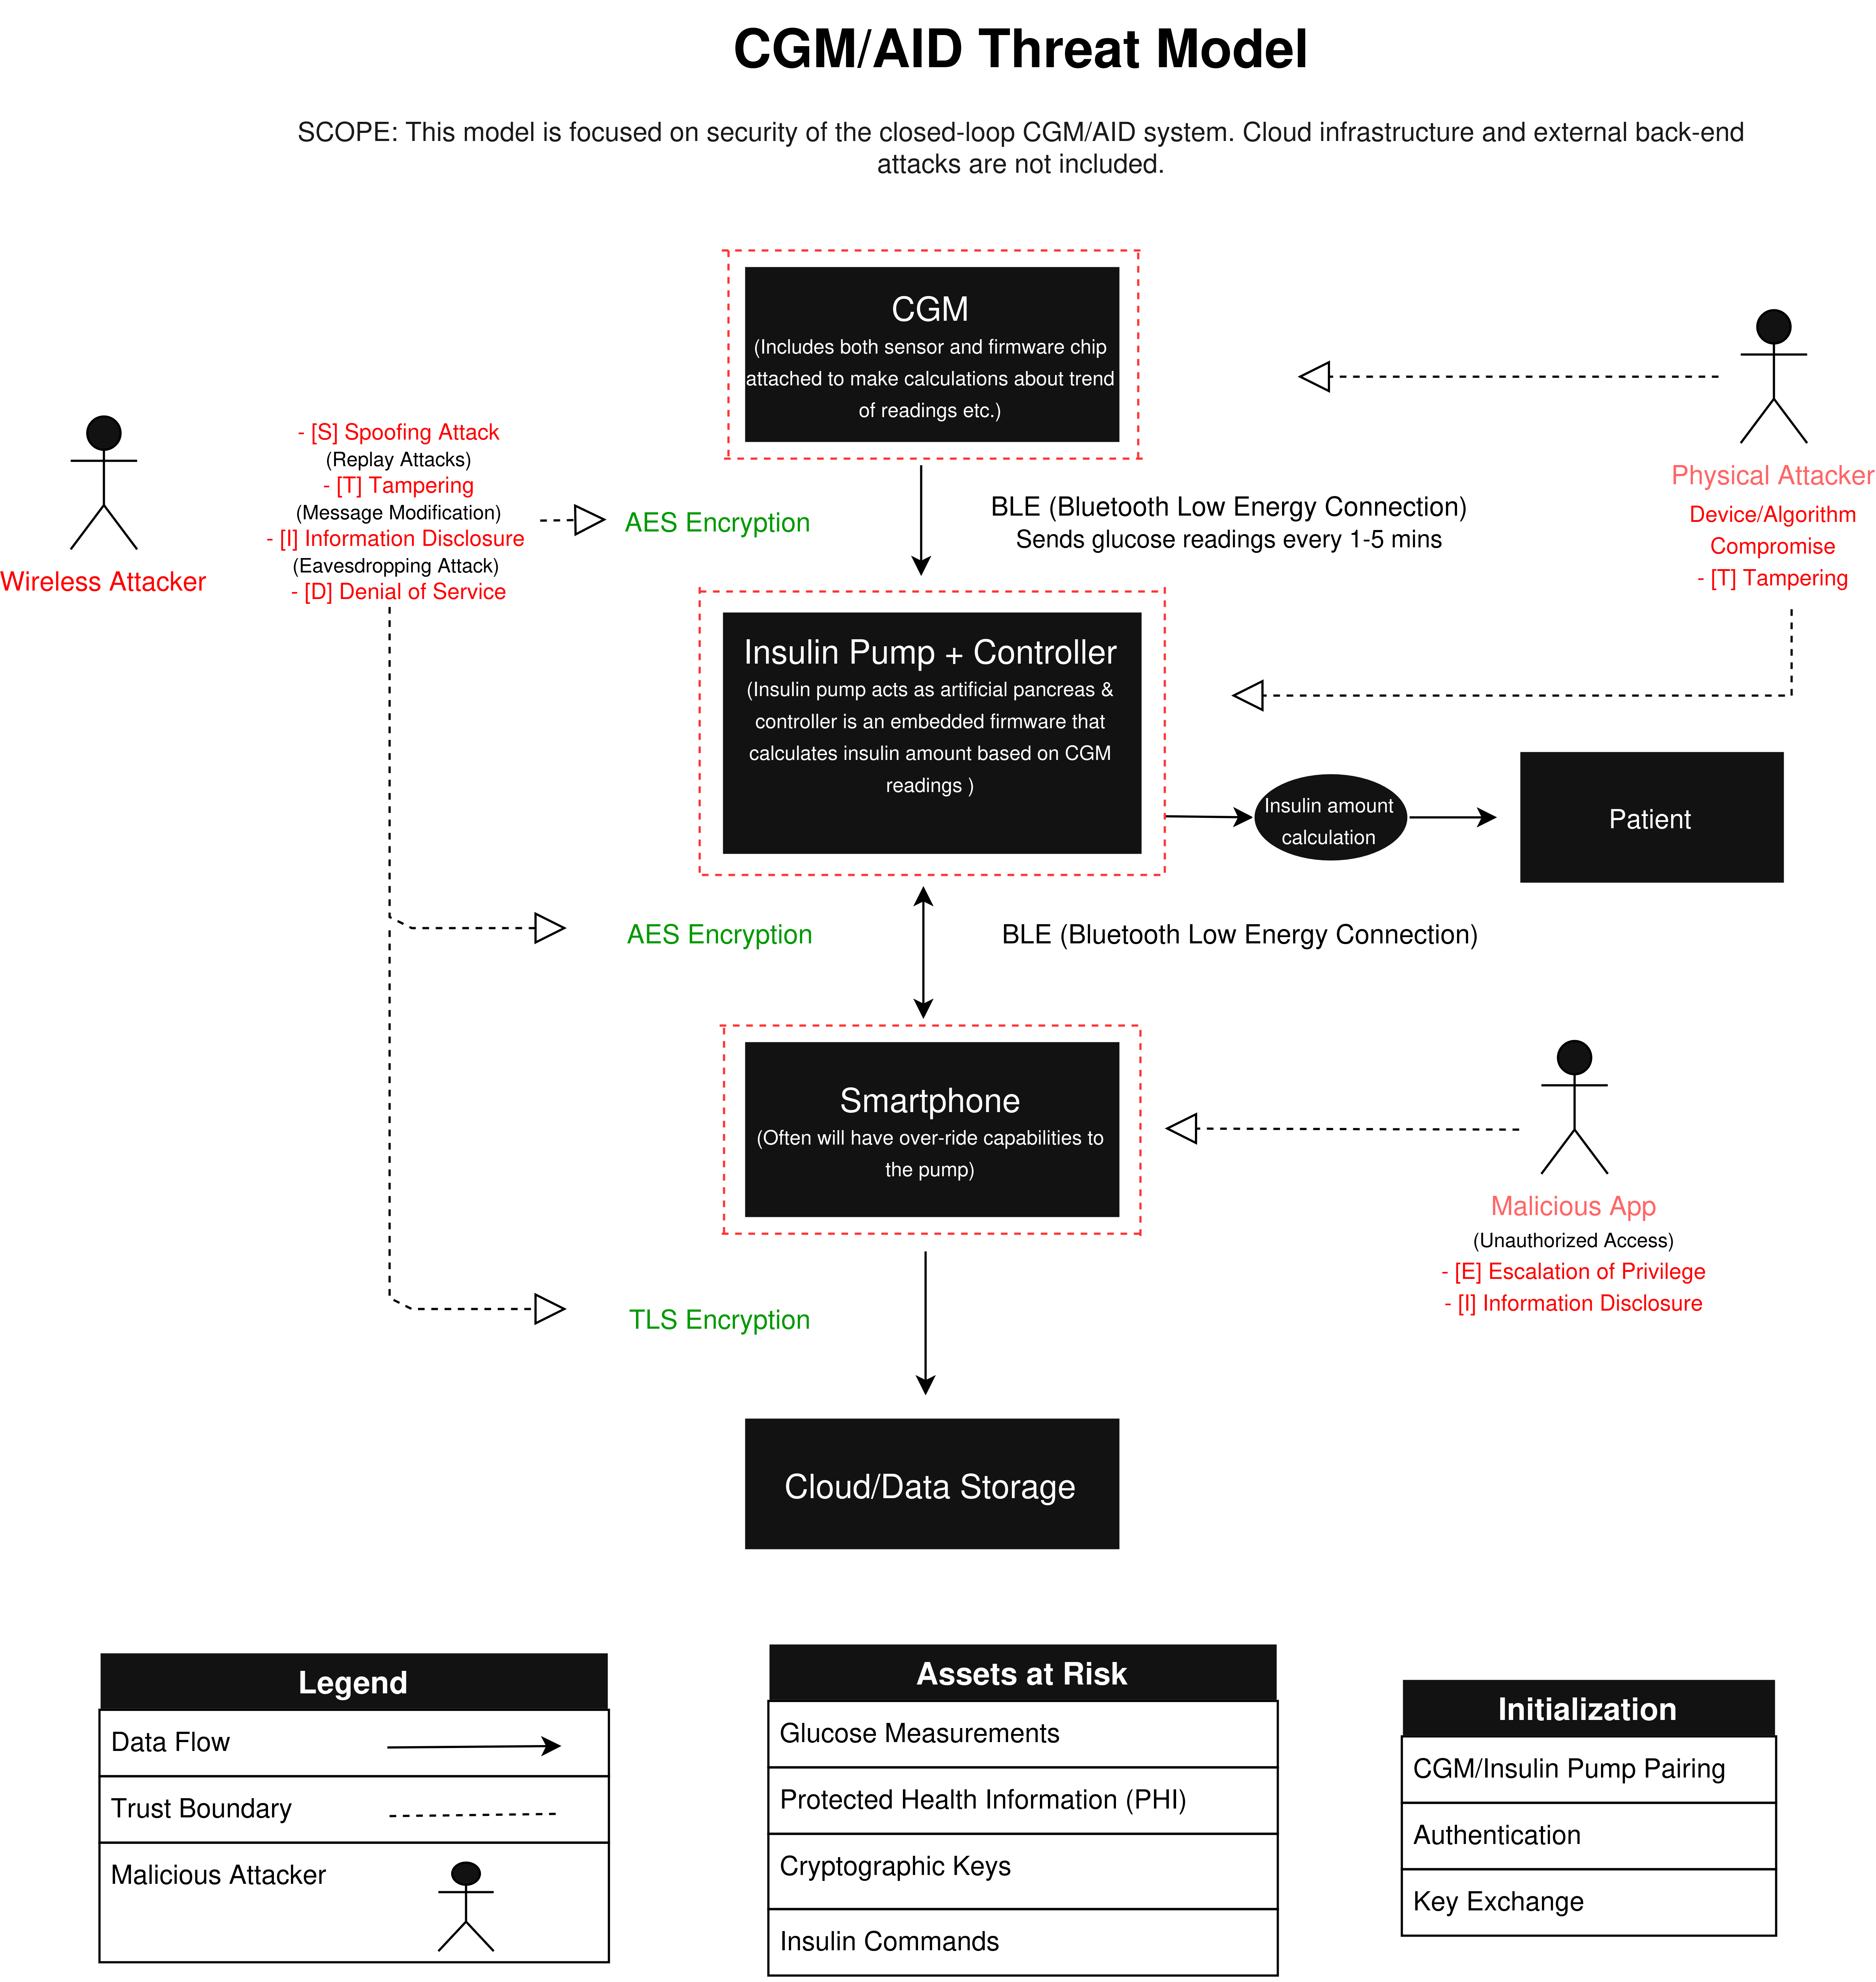
\includegraphics[width=1.0\linewidth]{STRIDEThreatModelPaper.png}
    \caption{STRIDE Threat Model}
    \label{fig:placeholder}
\end{figure}


\subsection{Scope \& Assumptions}
This simulation of a CGM/AID system focused specifically on the communication between the CGM and the insulin pump/controller, and excludes connection to the smartphone/mobile device and cloud/database.

\subsubsection{Inside Scope}
\begin{itemize}
    \item CGM \& AID communication
    \item  Symmetric encryption protocols for messages/glucose readings
    \item Computational overhead for encryption algorithms
    \item Security requirements derived from STRIDE \& STPA Sec frameworks
\end{itemize}

\subsubsection{Outside Scope}
\begin{itemize}
    \item BLE connection reliability
    \item Connection to smartphone/mobile devices
    \item Data storage in cloud/hospital system
\end{itemize}

\subsubsection{Assumptions}
\begin{itemize}
    \item Simulation is conducted on computer hardware rather than embedded hardware of artificial pancreas system - results are a relative comparison
    \item All encryption algorithms are implemented correctly in Python libraries
\end{itemize}
\subsection{Simulation Format}\label{AA}
The simulation of the CGM/AID system was done exclusively in Python. A list of the different programs and their purposes are listed below:
\begin{itemize}
\item \texttt{sample\_messages.json}: Acts as a predefined set of readings/messages to be encrypted and sent to the AID - includes glucose level, trend, timestamp, and reading ID
\item \texttt{sensor.py}:  Represents one session of the CGM device, by exchanging keys/pairing with the insulin pump, receiving a reading, and encrypting the message
\item \texttt{insulin\_pump.py}: Represents insulin pump by exchanging keys with CGM, and decrypting the message
\item \texttt{encryption.py}: Module for various encryption algorithms used in this simulation (Uses the cryptography.hazmat module)
\item \texttt{communication\_channel.py}: Simulates the communication channel between the CGM and AID - in most hardware systems today this is a Bluetooth Low Energy (BLE) connection 
\item \texttt{main.py}: This is the program that orchestrates full sessions of the CGM/AID by starting with an asymmetric key exchange (ECDH) and then using the various symmetric encryption algorithms for communication of different readings
\end{itemize}
\subsection{Benchmarking Metrics}
\begin{itemize}
    \item Latency: 
    \item Memory: measured using python module memray
\end{itemize}
\subsection{STPA-Sec Analysis}
\textbf{Identifying Losses}\\
In STPA losses are defined as "something of value to stakeholders" [cite]. The primary stakeholders in this system are the patient, healthcare provider, and system manufacturers. The losses identified are below.
\begin{itemize}
    \item L1: Loss of life/harm to patient health
    \item L2: Loss of device function/medical efficacy
    \item L3: Damage to device
    \item L4: Loss of patient data/PII
    \item L5: Loss of customer satisfaction
\end{itemize}

\textbf{Identifying System-level Hazards}\\
System-level hazards identify system state that with worst-case conditions will result in one or more losses identified above.
\begin{itemize}
    \item H1: Pump acts on incorrect/tampered/missing glucose readings [L1, L2]
    \item H2: Glucose readings are exposed to malicious attackers [L4, L5]
    \item H3: The pump is flooded with numerous glucose readings/excessive traffic [L1, L2]
    \item H4: Device hardware/computational resources are fully depleted [L2, L3]
\end{itemize}
\textbf{Identifying System-level Constraints}\\
Essentially, a system-level constraint aligns with a hazard to specify controls/conditions that must be put in place to avoid hazards.
\begin{itemize}
    \item SC-1: 
    \item SC-2:
    \item SC-3:
    \item SC-4:
\end{itemize}

\textbf{Control Structure}\\
A control structure was then developed based on the controllers, feedback loops, and control actions. Certain elements of this system have been abstracted in order to remain in scope and reduce complexity.
\begin{figure}[H]
    \centering
    
\includegraphics[width=1.0\linewidth]{STPAControlStructure.pdf}
    \caption{Hierarchical STPA Control Structure}
    \label{fig:placeholder}
\end{figure}
\textbf{Unsafe Control Actions (UCAs)}\\
\begin{table}[H]
    %\caption{}
    \centering
    \begin{tabularx}{\linewidth}{|X|X|X|X|X|}
        \hline
        \textbf{Control Action} & \textbf{Not providing causes hazard} & \textbf{Providing causes hazard} &\textbf{Incorrect timing or order} & \textbf{Stopped or Applied Too Long} \\
        \hline
        Transmission of Glucose Reading & Reading blocked from being transmitted & Reading is tampered & Replayed reading & Controller flooded with readings-DDoS \\
        \hline
        Sensor reading glucose levels & Sensor unable to identify glucose level & - & - & - \\
        \hline
        Glucose data/trends to patient device & - & - & - & -\\
        \hline
        Insulin delivery to patient & Insulin is not sent via actuator to patient & - & - & - \\
        \hline
        Patient override to controller commands & - & - & - & -\\
        \hline
    \end{tabularx}
    %\label{tab1}
    
\end{table}

\section{Results}
\subsection{Computational Overhead Results}
\begin{figure}[H]
    \centering
    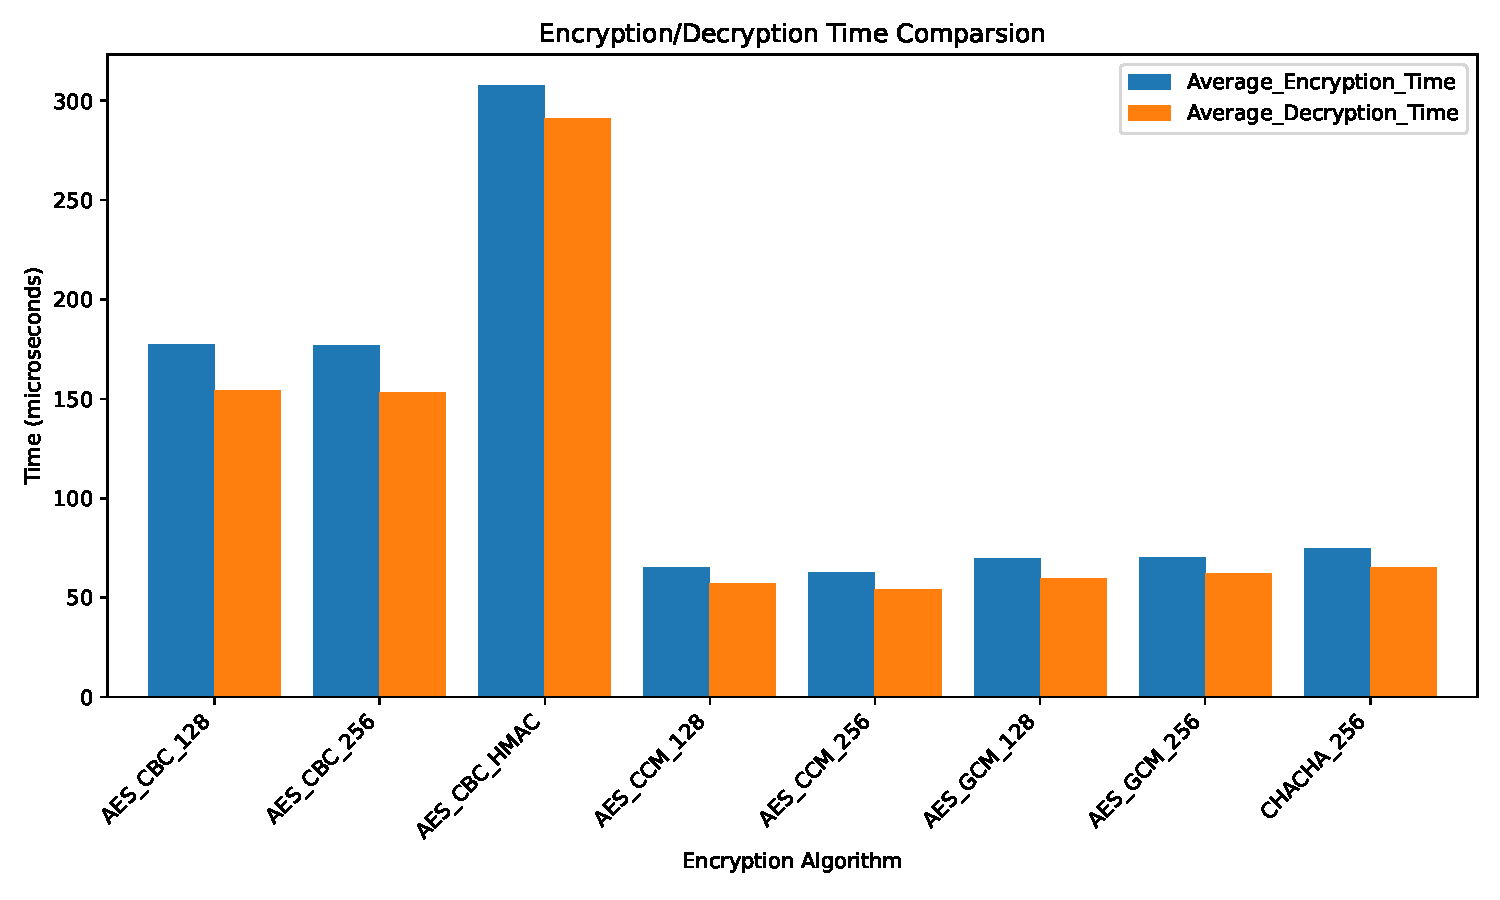
\includegraphics[width=1\linewidth]{TimeBenchmark.pdf}
    \caption{Time Benchmark Results}
    \label{fig:placeholder}
\end{figure}
The clear outlier here is CBC-HMAC, followed by the CBC encryption algorithm. This is likely due to the fact that CBC-HMAC is completing to seperate algorithms - one for CBC itself (which already has a relatively high latency when compared to other encryption methods) and one for the authentication via HMAC (hashing). All modern day algorithms (AES-CCM, AES-GCM, ChaCha20Poly1305) are all well optimized for time when compared to the legacy encryption algorithms, however AES-CCM has the lowest latency followeed by GCM and the ChaCha algorithm. 

\begin{figure}[H]
    \centering
    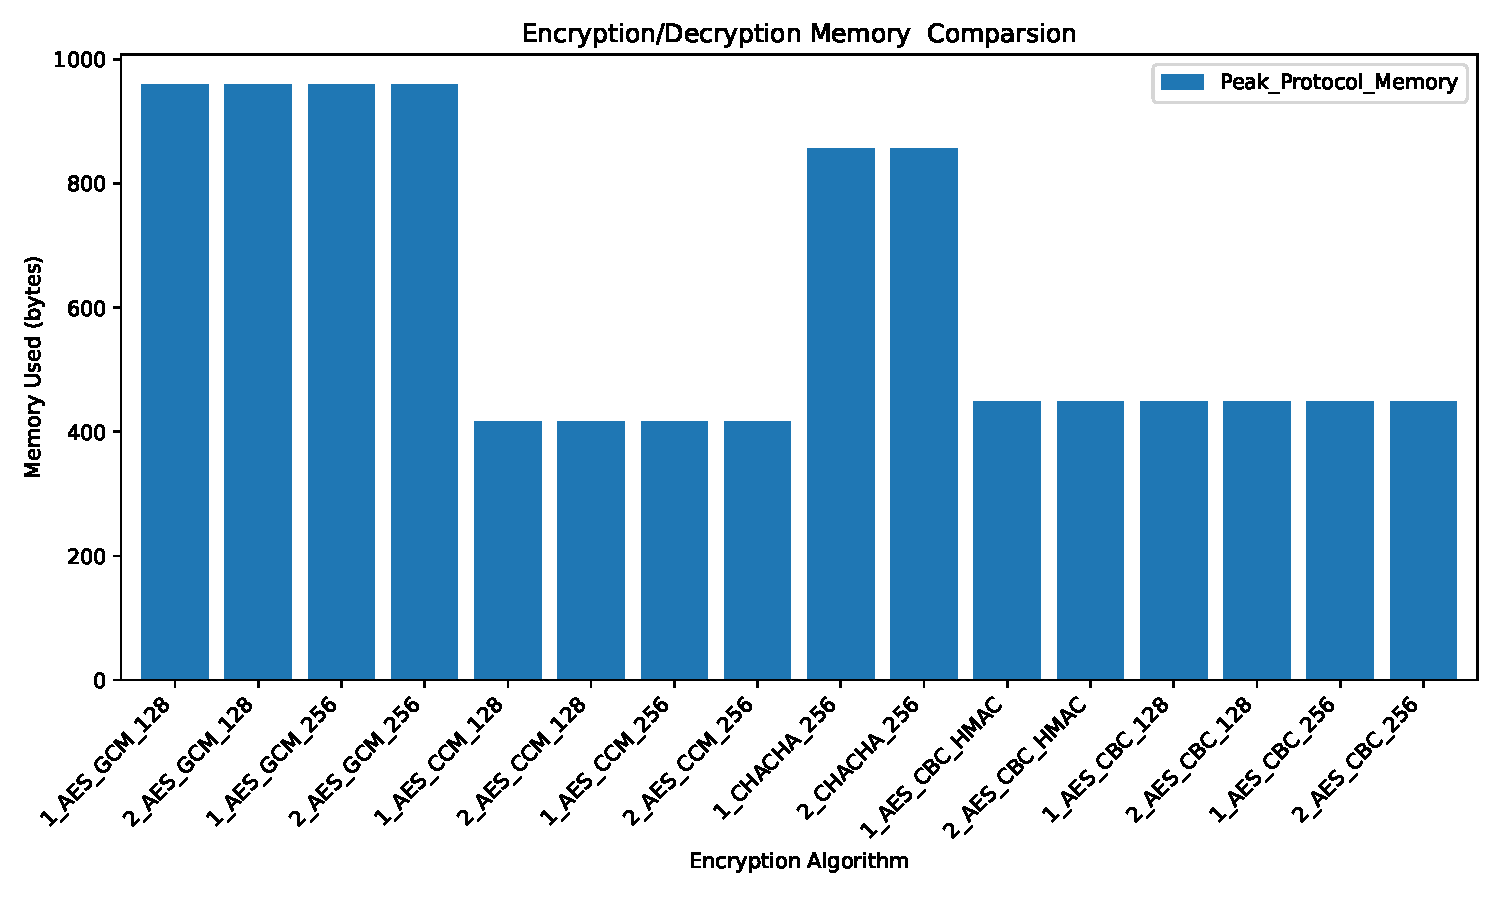
\includegraphics[width=1\linewidth]{MemoryBenchmark.pdf}
    \caption{Memory Benchmark Results}
    \label{fig:placeholder}
\end{figure}
The memory benchmark shows that AES-GCM \& the ChaCha algorithm have the highest memory overhead, with AES-CCM using the lowest. This specific graph does not show significant differences between different key sizes, there will be a computational overhead in terms of storing the additional key/ciphertext bits for the small embedded systems.

\section{Discussion}
\subsection{Key Takeaways}
\subsection{AES Accelerators}
One thing to note when discussing the implementation of these algorithms in an embedded system versus computer hardware is the presence of AES accelerators. Most modern day computer hardware (including the computer the simulation was run on) have AES accelerators, which significantly improves the time/computational overhead of AES based encryption systems. While many modern day artifical pancreas systems do have some form of an AES accelerator, in systems that do not have this compoenent, we may see that the ChaCha algorithm proves to be the superior choice.
\subsection{Limitations}
The largest limitation of this study is its inability to give results accurate to how encryption algorithms will work on an embedded systems device/actual artifical pancreas system. 

\section{Conclusion}

\subsection{Future Work}
Following this simulation, the next obvious step would be to take this simulation and implement it in a embedded systems device to better simulate the CGM/AID system. Additionally, expanding this simulation to analyze different forms of key exchange/asymmetric encryption algorithms will provide insight into that portion of the encryption process. 

\section*{Acknowledgment}

This research was done as a part of the summer internship at the Institute for Computing in Research. All work and resources used were open source as per institute policy.
\newpage
%\section{References}
\bibliographystyle{IEEEtran}
\nocite{*}
\bibliography{references}
\end{document}
